\documentclass[11pt]{article}

    \usepackage[breakable]{tcolorbox}
    \usepackage{parskip} % Stop auto-indenting (to mimic markdown behaviour)
    

    % Basic figure setup, for now with no caption control since it's done
    % automatically by Pandoc (which extracts ![](path) syntax from Markdown).
    \usepackage{graphicx}
    % Maintain compatibility with old templates. Remove in nbconvert 6.0
    \let\Oldincludegraphics\includegraphics
    % Ensure that by default, figures have no caption (until we provide a
    % proper Figure object with a Caption API and a way to capture that
    % in the conversion process - todo).
    \usepackage{caption}
    %\DeclareCaptionFormat{nocaption}{}
    %\captionsetup{format=nocaption,aboveskip=0pt,belowskip=0pt}

    \usepackage{float}
    \floatplacement{figure}{H} % forces figures to be placed at the correct location
    \usepackage{xcolor} % Allow colors to be defined
    \usepackage{enumerate} % Needed for markdown enumerations to work
    \usepackage{geometry} % Used to adjust the document margins
    \usepackage{amsmath} % Equations
    \usepackage{amssymb} % Equations
    \usepackage{textcomp} % defines textquotesingle
    % Hack from http://tex.stackexchange.com/a/47451/13684:
    \AtBeginDocument{%
        \def\PYZsq{\textquotesingle}% Upright quotes in Pygmentized code
    }
    \usepackage{upquote} % Upright quotes for verbatim code
    \usepackage{eurosym} % defines \euro

    \usepackage{iftex}
    \ifPDFTeX
        \usepackage[T1]{fontenc}
        \IfFileExists{alphabeta.sty}{
              \usepackage{alphabeta}
          }{
              \usepackage[mathletters]{ucs}
              \usepackage[utf8x]{inputenc}
          }
    \else
        \usepackage{fontspec}
        \usepackage{unicode-math}
    \fi

    \usepackage{fancyvrb} % verbatim replacement that allows latex
    \usepackage{grffile} % extends the file name processing of package graphics 
                         % to support a larger range
    \makeatletter % fix for old versions of grffile with XeLaTeX
    \@ifpackagelater{grffile}{2019/11/01}
    {
      % Do nothing on new versions
    }
    {
      \def\Gread@@xetex#1{%
        \IfFileExists{"\Gin@base".bb}%
        {\Gread@eps{\Gin@base.bb}}%
        {\Gread@@xetex@aux#1}%
      }
    }
    \makeatother
    \usepackage[Export]{adjustbox} % Used to constrain images to a maximum size
    \adjustboxset{max size={0.9\linewidth}{0.9\paperheight}}

    % The hyperref package gives us a pdf with properly built
    % internal navigation ('pdf bookmarks' for the table of contents,
    % internal cross-reference links, web links for URLs, etc.)
    \usepackage{hyperref}
    % The default LaTeX title has an obnoxious amount of whitespace. By default,
    % titling removes some of it. It also provides customization options.
    \usepackage{titling}
    \usepackage{longtable} % longtable support required by pandoc >1.10
    \usepackage{booktabs}  % table support for pandoc > 1.12.2
    \usepackage{array}     % table support for pandoc >= 2.11.3
    \usepackage{calc}      % table minipage width calculation for pandoc >= 2.11.1
    \usepackage[inline]{enumitem} % IRkernel/repr support (it uses the enumerate* environment)
    \usepackage[normalem]{ulem} % ulem is needed to support strikethroughs (\sout)
                                % normalem makes italics be italics, not underlines
    \usepackage{mathrsfs}
    \usepackage{listings}
    \definecolor{codegreen}{rgb}{0,0.6,0}
    \definecolor{codegray}{rgb}{0.5,0.5,0.5}
    \definecolor{codepurple}{rgb}{0.58,0,0.82}
    \definecolor{backcolour}{rgb}{0.95,0.95,0.92}
    
    \lstdefinestyle{mystyle}{
        backgroundcolor=\color{backcolour},   
        commentstyle=\color{codegreen},
        keywordstyle=\color{magenta},
        numberstyle=\tiny\color{codegray},
        stringstyle=\color{codepurple},
        basicstyle=\ttfamily\footnotesize,
        breakatwhitespace=false,         
        breaklines=true,                 
        captionpos=b,                    
        keepspaces=true,                 
        numbers=left,                    
        numbersep=5pt,                  
        showspaces=false,                
        showstringspaces=false,
        showtabs=false,                  
        tabsize=2
    }
    
    \lstset{style=mystyle}
    

    
    % Colors for the hyperref package
    \definecolor{urlcolor}{rgb}{0,.145,.698}
    \definecolor{linkcolor}{rgb}{.71,0.21,0.01}
    \definecolor{citecolor}{rgb}{.12,.54,.11}

    % ANSI colors
    \definecolor{ansi-black}{HTML}{3E424D}
    \definecolor{ansi-black-intense}{HTML}{282C36}
    \definecolor{ansi-red}{HTML}{E75C58}
    \definecolor{ansi-red-intense}{HTML}{B22B31}
    \definecolor{ansi-green}{HTML}{00A250}
    \definecolor{ansi-green-intense}{HTML}{007427}
    \definecolor{ansi-yellow}{HTML}{DDB62B}
    \definecolor{ansi-yellow-intense}{HTML}{B27D12}
    \definecolor{ansi-blue}{HTML}{208FFB}
    \definecolor{ansi-blue-intense}{HTML}{0065CA}
    \definecolor{ansi-magenta}{HTML}{D160C4}
    \definecolor{ansi-magenta-intense}{HTML}{A03196}
    \definecolor{ansi-cyan}{HTML}{60C6C8}
    \definecolor{ansi-cyan-intense}{HTML}{258F8F}
    \definecolor{ansi-white}{HTML}{C5C1B4}
    \definecolor{ansi-white-intense}{HTML}{A1A6B2}
    \definecolor{ansi-default-inverse-fg}{HTML}{FFFFFF}
    \definecolor{ansi-default-inverse-bg}{HTML}{000000}

    % common color for the border for error outputs.
    \definecolor{outerrorbackground}{HTML}{FFDFDF}

    % commands and environments needed by pandoc snippets
    % extracted from the output of `pandoc -s`
    \providecommand{\tightlist}{%
      \setlength{\itemsep}{0pt}\setlength{\parskip}{0pt}}
    \DefineVerbatimEnvironment{Highlighting}{Verbatim}{commandchars=\\\{\}}
    % Add ',fontsize=\small' for more characters per line
    \newenvironment{Shaded}{}{}
    \newcommand{\KeywordTok}[1]{\textcolor[rgb]{0.00,0.44,0.13}{\textbf{{#1}}}}
    \newcommand{\DataTypeTok}[1]{\textcolor[rgb]{0.56,0.13,0.00}{{#1}}}
    \newcommand{\DecValTok}[1]{\textcolor[rgb]{0.25,0.63,0.44}{{#1}}}
    \newcommand{\BaseNTok}[1]{\textcolor[rgb]{0.25,0.63,0.44}{{#1}}}
    \newcommand{\FloatTok}[1]{\textcolor[rgb]{0.25,0.63,0.44}{{#1}}}
    \newcommand{\CharTok}[1]{\textcolor[rgb]{0.25,0.44,0.63}{{#1}}}
    \newcommand{\StringTok}[1]{\textcolor[rgb]{0.25,0.44,0.63}{{#1}}}
    \newcommand{\CommentTok}[1]{\textcolor[rgb]{0.38,0.63,0.69}{\textit{{#1}}}}
    \newcommand{\OtherTok}[1]{\textcolor[rgb]{0.00,0.44,0.13}{{#1}}}
    \newcommand{\AlertTok}[1]{\textcolor[rgb]{1.00,0.00,0.00}{\textbf{{#1}}}}
    \newcommand{\FunctionTok}[1]{\textcolor[rgb]{0.02,0.16,0.49}{{#1}}}
    \newcommand{\RegionMarkerTok}[1]{{#1}}
    \newcommand{\ErrorTok}[1]{\textcolor[rgb]{1.00,0.00,0.00}{\textbf{{#1}}}}
    \newcommand{\NormalTok}[1]{{#1}}
    
    % Additional commands for more recent versions of Pandoc
    \newcommand{\ConstantTok}[1]{\textcolor[rgb]{0.53,0.00,0.00}{{#1}}}
    \newcommand{\SpecialCharTok}[1]{\textcolor[rgb]{0.25,0.44,0.63}{{#1}}}
    \newcommand{\VerbatimStringTok}[1]{\textcolor[rgb]{0.25,0.44,0.63}{{#1}}}
    \newcommand{\SpecialStringTok}[1]{\textcolor[rgb]{0.73,0.40,0.53}{{#1}}}
    \newcommand{\ImportTok}[1]{{#1}}
    \newcommand{\DocumentationTok}[1]{\textcolor[rgb]{0.73,0.13,0.13}{\textit{{#1}}}}
    \newcommand{\AnnotationTok}[1]{\textcolor[rgb]{0.38,0.63,0.69}{\textbf{\textit{{#1}}}}}
    \newcommand{\CommentVarTok}[1]{\textcolor[rgb]{0.38,0.63,0.69}{\textbf{\textit{{#1}}}}}
    \newcommand{\VariableTok}[1]{\textcolor[rgb]{0.10,0.09,0.49}{{#1}}}
    \newcommand{\ControlFlowTok}[1]{\textcolor[rgb]{0.00,0.44,0.13}{\textbf{{#1}}}}
    \newcommand{\OperatorTok}[1]{\textcolor[rgb]{0.40,0.40,0.40}{{#1}}}
    \newcommand{\BuiltInTok}[1]{{#1}}
    \newcommand{\ExtensionTok}[1]{{#1}}
    \newcommand{\PreprocessorTok}[1]{\textcolor[rgb]{0.74,0.48,0.00}{{#1}}}
    \newcommand{\AttributeTok}[1]{\textcolor[rgb]{0.49,0.56,0.16}{{#1}}}
    \newcommand{\InformationTok}[1]{\textcolor[rgb]{0.38,0.63,0.69}{\textbf{\textit{{#1}}}}}
    \newcommand{\WarningTok}[1]{\textcolor[rgb]{0.38,0.63,0.69}{\textbf{\textit{{#1}}}}}
    
    
    % Define a nice break command that doesn't care if a line doesn't already
    % exist.
    \def\br{\hspace*{\fill} \\* }
    % Math Jax compatibility definitions
    \def\gt{>}
    \def\lt{<}
    \let\Oldtex\TeX
    \let\Oldlatex\LaTeX
    \renewcommand{\TeX}{\textrm{\Oldtex}}
    \renewcommand{\LaTeX}{\textrm{\Oldlatex}}
    % Document parameters
    % Document title
    \title{PEC 2}
    
    
    
    
    
% Pygments definitions
\makeatletter
\def\PY@reset{\let\PY@it=\relax \let\PY@bf=\relax%
    \let\PY@ul=\relax \let\PY@tc=\relax%
    \let\PY@bc=\relax \let\PY@ff=\relax}
\def\PY@tok#1{\csname PY@tok@#1\endcsname}
\def\PY@toks#1+{\ifx\relax#1\empty\else%
    \PY@tok{#1}\expandafter\PY@toks\fi}
\def\PY@do#1{\PY@bc{\PY@tc{\PY@ul{%
    \PY@it{\PY@bf{\PY@ff{#1}}}}}}}
\def\PY#1#2{\PY@reset\PY@toks#1+\relax+\PY@do{#2}}

\@namedef{PY@tok@w}{\def\PY@tc##1{\textcolor[rgb]{0.73,0.73,0.73}{##1}}}
\@namedef{PY@tok@c}{\let\PY@it=\textit\def\PY@tc##1{\textcolor[rgb]{0.24,0.48,0.48}{##1}}}
\@namedef{PY@tok@cp}{\def\PY@tc##1{\textcolor[rgb]{0.61,0.40,0.00}{##1}}}
\@namedef{PY@tok@k}{\let\PY@bf=\textbf\def\PY@tc##1{\textcolor[rgb]{0.00,0.50,0.00}{##1}}}
\@namedef{PY@tok@kp}{\def\PY@tc##1{\textcolor[rgb]{0.00,0.50,0.00}{##1}}}
\@namedef{PY@tok@kt}{\def\PY@tc##1{\textcolor[rgb]{0.69,0.00,0.25}{##1}}}
\@namedef{PY@tok@o}{\def\PY@tc##1{\textcolor[rgb]{0.40,0.40,0.40}{##1}}}
\@namedef{PY@tok@ow}{\let\PY@bf=\textbf\def\PY@tc##1{\textcolor[rgb]{0.67,0.13,1.00}{##1}}}
\@namedef{PY@tok@nb}{\def\PY@tc##1{\textcolor[rgb]{0.00,0.50,0.00}{##1}}}
\@namedef{PY@tok@nf}{\def\PY@tc##1{\textcolor[rgb]{0.00,0.00,1.00}{##1}}}
\@namedef{PY@tok@nc}{\let\PY@bf=\textbf\def\PY@tc##1{\textcolor[rgb]{0.00,0.00,1.00}{##1}}}
\@namedef{PY@tok@nn}{\let\PY@bf=\textbf\def\PY@tc##1{\textcolor[rgb]{0.00,0.00,1.00}{##1}}}
\@namedef{PY@tok@ne}{\let\PY@bf=\textbf\def\PY@tc##1{\textcolor[rgb]{0.80,0.25,0.22}{##1}}}
\@namedef{PY@tok@nv}{\def\PY@tc##1{\textcolor[rgb]{0.10,0.09,0.49}{##1}}}
\@namedef{PY@tok@no}{\def\PY@tc##1{\textcolor[rgb]{0.53,0.00,0.00}{##1}}}
\@namedef{PY@tok@nl}{\def\PY@tc##1{\textcolor[rgb]{0.46,0.46,0.00}{##1}}}
\@namedef{PY@tok@ni}{\let\PY@bf=\textbf\def\PY@tc##1{\textcolor[rgb]{0.44,0.44,0.44}{##1}}}
\@namedef{PY@tok@na}{\def\PY@tc##1{\textcolor[rgb]{0.41,0.47,0.13}{##1}}}
\@namedef{PY@tok@nt}{\let\PY@bf=\textbf\def\PY@tc##1{\textcolor[rgb]{0.00,0.50,0.00}{##1}}}
\@namedef{PY@tok@nd}{\def\PY@tc##1{\textcolor[rgb]{0.67,0.13,1.00}{##1}}}
\@namedef{PY@tok@s}{\def\PY@tc##1{\textcolor[rgb]{0.73,0.13,0.13}{##1}}}
\@namedef{PY@tok@sd}{\let\PY@it=\textit\def\PY@tc##1{\textcolor[rgb]{0.73,0.13,0.13}{##1}}}
\@namedef{PY@tok@si}{\let\PY@bf=\textbf\def\PY@tc##1{\textcolor[rgb]{0.64,0.35,0.47}{##1}}}
\@namedef{PY@tok@se}{\let\PY@bf=\textbf\def\PY@tc##1{\textcolor[rgb]{0.67,0.36,0.12}{##1}}}
\@namedef{PY@tok@sr}{\def\PY@tc##1{\textcolor[rgb]{0.64,0.35,0.47}{##1}}}
\@namedef{PY@tok@ss}{\def\PY@tc##1{\textcolor[rgb]{0.10,0.09,0.49}{##1}}}
\@namedef{PY@tok@sx}{\def\PY@tc##1{\textcolor[rgb]{0.00,0.50,0.00}{##1}}}
\@namedef{PY@tok@m}{\def\PY@tc##1{\textcolor[rgb]{0.40,0.40,0.40}{##1}}}
\@namedef{PY@tok@gh}{\let\PY@bf=\textbf\def\PY@tc##1{\textcolor[rgb]{0.00,0.00,0.50}{##1}}}
\@namedef{PY@tok@gu}{\let\PY@bf=\textbf\def\PY@tc##1{\textcolor[rgb]{0.50,0.00,0.50}{##1}}}
\@namedef{PY@tok@gd}{\def\PY@tc##1{\textcolor[rgb]{0.63,0.00,0.00}{##1}}}
\@namedef{PY@tok@gi}{\def\PY@tc##1{\textcolor[rgb]{0.00,0.52,0.00}{##1}}}
\@namedef{PY@tok@gr}{\def\PY@tc##1{\textcolor[rgb]{0.89,0.00,0.00}{##1}}}
\@namedef{PY@tok@ge}{\let\PY@it=\textit}
\@namedef{PY@tok@gs}{\let\PY@bf=\textbf}
\@namedef{PY@tok@gp}{\let\PY@bf=\textbf\def\PY@tc##1{\textcolor[rgb]{0.00,0.00,0.50}{##1}}}
\@namedef{PY@tok@go}{\def\PY@tc##1{\textcolor[rgb]{0.44,0.44,0.44}{##1}}}
\@namedef{PY@tok@gt}{\def\PY@tc##1{\textcolor[rgb]{0.00,0.27,0.87}{##1}}}
\@namedef{PY@tok@err}{\def\PY@bc##1{{\setlength{\fboxsep}{\string -\fboxrule}\fcolorbox[rgb]{1.00,0.00,0.00}{1,1,1}{\strut ##1}}}}
\@namedef{PY@tok@kc}{\let\PY@bf=\textbf\def\PY@tc##1{\textcolor[rgb]{0.00,0.50,0.00}{##1}}}
\@namedef{PY@tok@kd}{\let\PY@bf=\textbf\def\PY@tc##1{\textcolor[rgb]{0.00,0.50,0.00}{##1}}}
\@namedef{PY@tok@kn}{\let\PY@bf=\textbf\def\PY@tc##1{\textcolor[rgb]{0.00,0.50,0.00}{##1}}}
\@namedef{PY@tok@kr}{\let\PY@bf=\textbf\def\PY@tc##1{\textcolor[rgb]{0.00,0.50,0.00}{##1}}}
\@namedef{PY@tok@bp}{\def\PY@tc##1{\textcolor[rgb]{0.00,0.50,0.00}{##1}}}
\@namedef{PY@tok@fm}{\def\PY@tc##1{\textcolor[rgb]{0.00,0.00,1.00}{##1}}}
\@namedef{PY@tok@vc}{\def\PY@tc##1{\textcolor[rgb]{0.10,0.09,0.49}{##1}}}
\@namedef{PY@tok@vg}{\def\PY@tc##1{\textcolor[rgb]{0.10,0.09,0.49}{##1}}}
\@namedef{PY@tok@vi}{\def\PY@tc##1{\textcolor[rgb]{0.10,0.09,0.49}{##1}}}
\@namedef{PY@tok@vm}{\def\PY@tc##1{\textcolor[rgb]{0.10,0.09,0.49}{##1}}}
\@namedef{PY@tok@sa}{\def\PY@tc##1{\textcolor[rgb]{0.73,0.13,0.13}{##1}}}
\@namedef{PY@tok@sb}{\def\PY@tc##1{\textcolor[rgb]{0.73,0.13,0.13}{##1}}}
\@namedef{PY@tok@sc}{\def\PY@tc##1{\textcolor[rgb]{0.73,0.13,0.13}{##1}}}
\@namedef{PY@tok@dl}{\def\PY@tc##1{\textcolor[rgb]{0.73,0.13,0.13}{##1}}}
\@namedef{PY@tok@s2}{\def\PY@tc##1{\textcolor[rgb]{0.73,0.13,0.13}{##1}}}
\@namedef{PY@tok@sh}{\def\PY@tc##1{\textcolor[rgb]{0.73,0.13,0.13}{##1}}}
\@namedef{PY@tok@s1}{\def\PY@tc##1{\textcolor[rgb]{0.73,0.13,0.13}{##1}}}
\@namedef{PY@tok@mb}{\def\PY@tc##1{\textcolor[rgb]{0.40,0.40,0.40}{##1}}}
\@namedef{PY@tok@mf}{\def\PY@tc##1{\textcolor[rgb]{0.40,0.40,0.40}{##1}}}
\@namedef{PY@tok@mh}{\def\PY@tc##1{\textcolor[rgb]{0.40,0.40,0.40}{##1}}}
\@namedef{PY@tok@mi}{\def\PY@tc##1{\textcolor[rgb]{0.40,0.40,0.40}{##1}}}
\@namedef{PY@tok@il}{\def\PY@tc##1{\textcolor[rgb]{0.40,0.40,0.40}{##1}}}
\@namedef{PY@tok@mo}{\def\PY@tc##1{\textcolor[rgb]{0.40,0.40,0.40}{##1}}}
\@namedef{PY@tok@ch}{\let\PY@it=\textit\def\PY@tc##1{\textcolor[rgb]{0.24,0.48,0.48}{##1}}}
\@namedef{PY@tok@cm}{\let\PY@it=\textit\def\PY@tc##1{\textcolor[rgb]{0.24,0.48,0.48}{##1}}}
\@namedef{PY@tok@cpf}{\let\PY@it=\textit\def\PY@tc##1{\textcolor[rgb]{0.24,0.48,0.48}{##1}}}
\@namedef{PY@tok@c1}{\let\PY@it=\textit\def\PY@tc##1{\textcolor[rgb]{0.24,0.48,0.48}{##1}}}
\@namedef{PY@tok@cs}{\let\PY@it=\textit\def\PY@tc##1{\textcolor[rgb]{0.24,0.48,0.48}{##1}}}

\def\PYZbs{\char`\\}
\def\PYZus{\char`\_}
\def\PYZob{\char`\{}
\def\PYZcb{\char`\}}
\def\PYZca{\char`\^}
\def\PYZam{\char`\&}
\def\PYZlt{\char`\<}
\def\PYZgt{\char`\>}
\def\PYZsh{\char`\#}
\def\PYZpc{\char`\%}
\def\PYZdl{\char`\$}
\def\PYZhy{\char`\-}
\def\PYZsq{\char`\'}
\def\PYZdq{\char`\"}
\def\PYZti{\char`\~}
% for compatibility with earlier versions
\def\PYZat{@}
\def\PYZlb{[}
\def\PYZrb{]}
\makeatother


    % For linebreaks inside Verbatim environment from package fancyvrb. 
    \makeatletter
        \newbox\Wrappedcontinuationbox 
        \newbox\Wrappedvisiblespacebox 
        \newcommand*\Wrappedvisiblespace {\textcolor{red}{\textvisiblespace}} 
        \newcommand*\Wrappedcontinuationsymbol {\textcolor{red}{\llap{\tiny$\m@th\hookrightarrow$}}} 
        \newcommand*\Wrappedcontinuationindent {3ex } 
        \newcommand*\Wrappedafterbreak {\kern\Wrappedcontinuationindent\copy\Wrappedcontinuationbox} 
        % Take advantage of the already applied Pygments mark-up to insert 
        % potential linebreaks for TeX processing. 
        %        {, <, #, %, $, ' and ": go to next line. 
        %        _, }, ^, &, >, - and ~: stay at end of broken line. 
        % Use of \textquotesingle for straight quote. 
        \newcommand*\Wrappedbreaksatspecials {% 
            \def\PYGZus{\discretionary{\char`\_}{\Wrappedafterbreak}{\char`\_}}% 
            \def\PYGZob{\discretionary{}{\Wrappedafterbreak\char`\{}{\char`\{}}% 
            \def\PYGZcb{\discretionary{\char`\}}{\Wrappedafterbreak}{\char`\}}}% 
            \def\PYGZca{\discretionary{\char`\^}{\Wrappedafterbreak}{\char`\^}}% 
            \def\PYGZam{\discretionary{\char`\&}{\Wrappedafterbreak}{\char`\&}}% 
            \def\PYGZlt{\discretionary{}{\Wrappedafterbreak\char`\<}{\char`\<}}% 
            \def\PYGZgt{\discretionary{\char`\>}{\Wrappedafterbreak}{\char`\>}}% 
            \def\PYGZsh{\discretionary{}{\Wrappedafterbreak\char`\#}{\char`\#}}% 
            \def\PYGZpc{\discretionary{}{\Wrappedafterbreak\char`\%}{\char`\%}}% 
            \def\PYGZdl{\discretionary{}{\Wrappedafterbreak\char`\$}{\char`\$}}% 
            \def\PYGZhy{\discretionary{\char`\-}{\Wrappedafterbreak}{\char`\-}}% 
            \def\PYGZsq{\discretionary{}{\Wrappedafterbreak\textquotesingle}{\textquotesingle}}% 
            \def\PYGZdq{\discretionary{}{\Wrappedafterbreak\char`\"}{\char`\"}}% 
            \def\PYGZti{\discretionary{\char`\~}{\Wrappedafterbreak}{\char`\~}}% 
        } 
        % Some characters . , ; ? ! / are not pygmentized. 
        % This macro makes them "active" and they will insert potential linebreaks 
        \newcommand*\Wrappedbreaksatpunct {% 
            \lccode`\~`\.\lowercase{\def~}{\discretionary{\hbox{\char`\.}}{\Wrappedafterbreak}{\hbox{\char`\.}}}% 
            \lccode`\~`\,\lowercase{\def~}{\discretionary{\hbox{\char`\,}}{\Wrappedafterbreak}{\hbox{\char`\,}}}% 
            \lccode`\~`\;\lowercase{\def~}{\discretionary{\hbox{\char`\;}}{\Wrappedafterbreak}{\hbox{\char`\;}}}% 
            \lccode`\~`\:\lowercase{\def~}{\discretionary{\hbox{\char`\:}}{\Wrappedafterbreak}{\hbox{\char`\:}}}% 
            \lccode`\~`\?\lowercase{\def~}{\discretionary{\hbox{\char`\?}}{\Wrappedafterbreak}{\hbox{\char`\?}}}% 
            \lccode`\~`\!\lowercase{\def~}{\discretionary{\hbox{\char`\!}}{\Wrappedafterbreak}{\hbox{\char`\!}}}% 
            \lccode`\~`\/\lowercase{\def~}{\discretionary{\hbox{\char`\/}}{\Wrappedafterbreak}{\hbox{\char`\/}}}% 
            \catcode`\.\active
            \catcode`\,\active 
            \catcode`\;\active
            \catcode`\:\active
            \catcode`\?\active
            \catcode`\!\active
            \catcode`\/\active 
            \lccode`\~`\~ 	
        }
    \makeatother

    \let\OriginalVerbatim=\Verbatim
    \makeatletter
    \renewcommand{\Verbatim}[1][1]{%
        %\parskip\z@skip
        \sbox\Wrappedcontinuationbox {\Wrappedcontinuationsymbol}%
        \sbox\Wrappedvisiblespacebox {\FV@SetupFont\Wrappedvisiblespace}%
        \def\FancyVerbFormatLine ##1{\hsize\linewidth
            \vtop{\raggedright\hyphenpenalty\z@\exhyphenpenalty\z@
                \doublehyphendemerits\z@\finalhyphendemerits\z@
                \strut ##1\strut}%
        }%
        % If the linebreak is at a space, the latter will be displayed as visible
        % space at end of first line, and a continuation symbol starts next line.
        % Stretch/shrink are however usually zero for typewriter font.
        \def\FV@Space {%
            \nobreak\hskip\z@ plus\fontdimen3\font minus\fontdimen4\font
            \discretionary{\copy\Wrappedvisiblespacebox}{\Wrappedafterbreak}
            {\kern\fontdimen2\font}%
        }%
        
        % Allow breaks at special characters using \PYG... macros.
        \Wrappedbreaksatspecials
        % Breaks at punctuation characters . , ; ? ! and / need catcode=\active 	
        \OriginalVerbatim[#1,codes*=\Wrappedbreaksatpunct]%
    }
    \makeatother

    % Exact colors from NB
    \definecolor{incolor}{HTML}{303F9F}
    \definecolor{outcolor}{HTML}{D84315}
    \definecolor{cellborder}{HTML}{CFCFCF}
    \definecolor{cellbackground}{HTML}{F7F7F7}
    
    % prompt
    \makeatletter
    \newcommand{\boxspacing}{\kern\kvtcb@left@rule\kern\kvtcb@boxsep}
    \makeatother
    \newcommand{\prompt}[4]{
        {\ttfamily\llap{{\color{#2}[#3]:\hspace{3pt}#4}}\vspace{-\baselineskip}}
    }
    

    
    % Prevent overflowing lines due to hard-to-break entities
    \sloppy 
    % Setup hyperref package
    \hypersetup{
      breaklinks=true,  % so long urls are correctly broken across lines
      colorlinks=true,
      urlcolor=urlcolor,
      linkcolor=linkcolor,
      citecolor=citecolor,
      }
    % Slightly bigger margins than the latex defaults
    
    \geometry{verbose,tmargin=1in,bmargin=1in,lmargin=1in,rmargin=1in}
    
    

\begin{document}
    \author{Pablo Riutort Grande}
    \maketitle
    
M0.534 - Chaotic Dynamical Systems

Master's Degree in Computational and Mathematical Engineering 

\hypertarget{section}{%
\section{}\label{section}}
 Use a calculator (*) to iterate each of the following functions using arbitrary
initial value and explain these results.
\begin{itemize}
    \item $f(x)$ = cos(x).
    \item $f(x)$ = sin(x).
    \item $f(x)$ = $\frac{1}{e}e^{x}$
    \item $f(x)$ = arctan(x)
\end{itemize}

For this exercise the program Listing \ref{lst:logistic} was developed.\\
Each function has its alias in the program:
\begin{itemize}
    \item $C(x) = cos(x)$
    \item $S(x) = sin(x)$
    \item $E(x)$ = $\frac{1}{e}e^{x}$
    \item $A(x)$ = arctan(x)
\end{itemize}
A random seed betwen 0 and 1 is generated and input to each function to iterate a total of 10. This process is repeated 5 times for each function, below the results of each function.

\begin{lstlisting}[language=python]
Iteration 1
C(x) where x = 0.4394000429439828
0.9050070457601522
0.6176800389550504
0.8152242441563745
0.6857051880005774
0.7739727011574452
0.7151394744642647
0.7550017919794308
0.7282703151583196
0.7463267613590441
0.7341877488586638

S(x) where x = 0.10831863821671817
0.108106946656864
0.10789649334334948
0.10768726624042986
0.10747925347561625
0.10727244333683801
0.10706682426966521
0.10686238487458972
0.10665911390436336
0.10645700026139174
0.10625603299518253

E(x) where x = 0.14815376781101597
0.4266265527327907
0.5636208827195786
0.6463726284449933
0.7021365546674693
0.742402711381613
0.7729064276570666
0.7968462160341325
0.8161527205721868
0.8320628672410064
0.8454069814184962

A(x) where x = 0.7821630397171593
0.6637697232168888
0.5859943448654147
0.5300575669848065
0.48740352104128126
0.45351974019306424
0.42577708640213974
0.4025286624518398
0.38268435599525746
0.3654905616139816
0.3504076767769953

Iteration 2
C(x) where x = 0.40408353637833005
0.9194631149957769
0.6062472158896082
0.8217920889969251
0.6809098340876435
0.7770002996659591
0.7130199638877244
0.7563899063369314
0.7273183529743692
0.7469600298157653
0.7337576462700917

S(x) where x = 0.12103375585888243
0.12073846488489588
0.12044532889593297
0.12015432177745117
0.11986541785617934
0.11957859189057092
0.11929381906150852
0.119011074963252
0.11873033559462273
0.11845157735041656
0.11817477701303872

E(x) where x = 0.4339815100326633
0.5677815723363696
0.6490675868837624
0.704031335531694
0.743810735359876
0.7739954649555553
0.7977144839868321
0.816861667557403
0.8326529648514928
0.845906001278853
0.8571914423250133

A(x) where x = 0.9009731526656969
0.7333524951029998
0.6327612955766867
0.564161013724129
0.5136503437006801
0.47450815453217604
0.4430469581726845
0.41705675146734844
0.3951234536105647
0.37629540161910224
0.35990588088318803

Iteration 3
C(x) where x = 0.6285563747354734
0.8088771702874691
0.6903112492993068
0.7710478558906934
0.7171808262002901
0.7536616590930818
0.7291880405431919
0.7457156277533824
0.734602538751447
0.7420972272079335
0.7370528007865726

S(x) where x = 0.7146786935006394
0.6553747664930188
0.6094564083350839
0.5724218216529139
0.5416693982224934
0.5155671319159577
0.493028340579581
0.4732957304702167
0.45582218924659973
0.44020070574346337
0.4261210453409806

E(x) where x = 0.8057304291931797
0.8234359000670495
0.8381450523916006
0.8505645720180248
0.8611940452617592
0.870396908468477
0.8784440236083432
0.8855414825446277
0.8918489338139864
0.8974920054948423
0.902570934116095

A(x) where x = 0.17674942307351982
0.17494259974994686
0.17318997130674557
0.17148888459607214
0.16983686468047773
0.168231599741146
0.16667092751862764
0.16515282310556223
0.163675387934966
0.1622368398281748
0.16083550398404664

Iteration 4
C(x) where x = 0.2544759469236577
0.9677953527894435
0.5671167378641422
0.8434533742165292
0.6648873195935878
0.7869863106064461
0.7059829002613517
0.7609742313504698
0.7241644979966512
0.749053211642457
0.732333908473518

S(x) where x = 0.41358938124712186
0.40189864942826004
0.3911664112866533
0.3812669806190342
0.37209677148492626
0.36356951301351464
0.3556126778371633
0.34816477518442357
0.3411732708611497
0.3345929689320985
0.3283847383133514

E(x) where x = 0.19409582858422603
0.446683865133747
0.5750397357810781
0.6537957636990407
0.7073680021282935
0.7462967289541846
0.7759220064161287
0.7992527953484465
0.8181192221487418
0.8337007300833409
0.8467927766614857

A(x) where x = 0.42287808301020735
0.4000719926983752
0.3805684382426265
0.3636436290679176
0.34877742048293375
0.3355852467680442
0.32377590544207613
0.313124349350273
0.30345356948168106
0.294622187483076
0.2865157482775393

Iteration 5
C(x) where x = 0.32538626283620975
0.9475273186063715
0.5836926265494049
0.8344333039924641
0.6715976646384912
0.7828285385855893
0.7089214438147813
0.7590644741048073
0.7254801973071787
0.7481808998265066
0.7329276267517787

S(x) where x = 0.7183583955499566
0.6581496164190729
0.6116540145223439
0.574222385592138
0.5431820582999441
0.5168626631371835
0.49415505584308866
0.47428795736996815
0.45670511696772204
0.44099331433279965
0.42683795758136756

E(x) where x = 0.4695949438487651
0.5883665998945722
0.6625671285740302
0.7135998760408172
0.7509620779048526
0.7795504106393188
0.8021580751438147
0.8204995434704858
0.8356875694270306
0.8484768903437631
0.8593980216505906

A(x) where x = 0.27972106068778824
0.27275002401623266
0.2662732252283477
0.2602350349355436
0.25458819856749637
0.2492922839947751
0.24431246663744724
0.2396185687055573
0.23518429208942865
0.23098660043122332
0.22700521728353343
\end{lstlisting}

This exercise consists in a fixed point iteration computation, for each function we will get a sequence of iterated function application and hopefully converge into a point called fixed point ($x_{fix}$).

\begin{itemize}
    \item $C(x) = cos(x)$ converges into 0.7341877488586638, 0.7337576462700917, 0.7370528007865726, 0.732333908473518, 0.7329276267517787 $\simeq$ 0.73.  
    \item $S(x) = sin(x)$ converges into 0.10625603299518253, 0.11817477701303872, 0.4261210453409806, 0.3283847383133514, 0.42683795758136756 don't seem to converge into any point. We can observe 2 similar points in 3rd and 5th iteration but this is because of similar initial seeds. Besides that, this function does not seem to converge into any given point.
    \item $E(x)$ = $\frac{1}{e}e^{x}$ converges into 0.8454069814184962, 0.8571914423250133, 0.902570934116095, 0.8467927766614857, 0.8593980216505906. In 3rd iteration we put a seed close to a, what it seems to be, fixed point, but all previous values are close to $\simeq$ 0.84.
    \item $A(x)$ = arctan(x) converges into 0.3504076767769953, 0.35990588088318803, 0.16083550398404664, 0.2865157482775393, 0.22700521728353343. Does not seem to converge into a fixed point but several.
\end{itemize}

\hypertarget{section}{%
\section{}\label{section}} Using the graph of the function, identify the fixed points for each of the maps in
the previous exercise.

To do this exercise the program Listing \ref{lst:plot} was developed. Below we have the result of the plot of each function with red points highlighting fixed points (Figure \ref{fig:cos}, Figure \ref{fig:sin}, Figure \ref{fig:e}, Figure \ref{fig:arctan}).

\hypertarget{3}{%
\section{}\label{3}} For $f(z) = z^{2} + \frac{5}{4}, z ∈ \mathbb{C}$ compute periodic orbits of period 1, 2 and 3.

To find the periodic orbits of period 1, 2, and 3 of the function $f(z) = z^2 + \frac{5}{4}$ we need to solve the equations:

\begin{equation}
    \begin{aligned}
    f(z) = z\\
    f(f(z)) = z\\
    f(f(f(z))) = z\\
    \end{aligned}
\end{equation}

\begin{center}
or
\end{center}

\begin{equation}
    \begin{gathered}
        z^2 + \frac{5}{4} = z\\
        (z^2 + \frac{5}{4})^2 + \frac{5}{4} = z\\
        ((z^2 + \frac{5}{4})^2 + \frac{5}{4})^2 +\frac{5}{4} = z
    \end{gathered}
\end{equation}

To do this exercise we will make use of Wolfram Alpha to compute these previous equations.

\begin{itemize}
    \item Period 1 solutions
    \begin{equation}
        \begin{gathered}
        z = \frac{1}{2} - i\\
        z = \frac{1}{2} + i
        \end{gathered}
    \end{equation}

    \item Period 2 solutions
    \begin{equation}
        \begin{gathered}
        z = \frac{1}{2} - i\\
        z = \frac{1}{2} + i\\
        z = -\frac{1}{2} - i \sqrt{2}\\
        z = -\frac{1}{2} + i \sqrt{2}
        \end{gathered}
    \end{equation}

    \item Period 3 solutions
    \begin{equation}
        \begin{gathered}
        z = \frac{1}{2} - i\\
        z = \frac{1}{2} + i\\
        z \simeq -0.64295 - 1.07015 i\\
        z \simeq -0.64295 + 1.07015 i\\
        z\simeq -0.3752 - 1.4261 i
        \end{gathered}
    \end{equation}
\end{itemize}


\hypertarget{4}{%
\section{}\label{4}}
Find all fixed points for each of the following maps and classify them as attracting,
repelling, or neither. Sketch the phase portraits.

To find fixed points we will solve the equation $f(x) = x$ and compute the derivative of the function at each fixed point to determine the behaviour. The behavior of the function near a fixed point is determined by the sign of the derivative at that point.\\
If:
\begin{itemize}
    \item $f'(x) < 1$ the point is an attractor or sink.
    \item $f'(x) > 1$ the point is a repellor or source.
    \item $f'(x) = 1$ the point is neither
\end{itemize}

Once all established we may begin our exercise.
\begin{itemize}
    \item  $f(x) = x − x^2$; $f'(x) = 1 - 2x$\\Has fixed point at $x=0$ and $f'(0) < 1$ hence it's attracting. Phase portrait in Figure \ref{fig:phase1}.
    \item  $f(x) = 2(x − x^2)$; $f'(x) = 2 - 4x$\\Has fixed points at $x=0$ and $x=\frac{1}{2}$. Phase portrait in Figure \ref{fig:phase2}.
        \begin{itemize}
            \item  $f'(0) = 2 > 1$. 0 is repelling
            \item  $f'(\frac{1}{2}) = 0 < 1$. $\frac{1}{2}$ is attracting
        \end{itemize}
    \item $f(x) = x^3 − \frac{1}{9}x$; $f'(x) = 3x^2 - \frac{1}{9}$\\Has fixed points at $x=0; x= - \frac{\sqrt{10}}{3}$ and $ x= \frac{\sqrt{10}}{3}$.  Phase portrait in Figure \ref{fig:phase3}.
        \begin{itemize}
            \item  $f'(0) = -\frac{1}{9} < 1$. 0 is attracting
            \item  $f'(-\frac{\sqrt{10}}{3}) = \frac{29}{9} > 1$. $-\frac{\sqrt{10}}{3}$ is repelling.
            \item  For $f'(\frac{\sqrt{10}}{3})$ we have the same result as above.
        \end{itemize}
    \item $f(x) = x^3 − x$; $f'(x) = 3x^2 - 1$\\Has fixed points at $x=0$ and $x= \pm \sqrt{2}$. Phase portrait in Figure \ref{fig:phase4}.
        \begin{itemize}
            \item  $f'(0) = -1 < 1$. 0 is attracting
            \item  $f'(\pm\sqrt{2}) = 5 > 1$. $\pm\sqrt{2}$ is repelling.
        \end{itemize}
    \item $S(x) = \frac{1}{2}sin(x)$; $f'(x) = \frac{1}{2}cos(x)$\\Has fixed point at $x = 0$ and $f'(0) = \frac{1}{2} < 1$ is attracting. Phase portrait in Figure \ref{fig:phase5}.
    \item $S(x) = sin(x)$; $f'(x) = cos(x)$\\Has fixed point at $x = 0$ and $f'(0) = 1$. 0 is neither attracting or repelling. Phase portrait in Figure \ref{fig:phase6}.
    \item $E(x) = e^{x-1}$; $f'(x) = e^{x-1}$\\Has fixed point at $x = 1$ and $f'(1) = 1$. 1 is neither attracting or repelling. Phase portrait in Figure \ref{fig:phase7}.
    \item $E(x) = e^x$; $f'(x) = e^x$\\Has no solution for $x \in \mathbb{R}$. Phase portrait in Figure \ref{fig:phase8}.
    \item $A(x) = arctan(x)$; $f'(x) = \frac{1}{x^2 +1}$\\Has fixed point at $x = 0$ and $f'(0) = 1$. 0 is neither attracting or repelling. Phase portrait in Figure \ref{fig:phase9}.
    \item $A(x) = \frac{\pi}{4}arctan(x)$; $f'(x) = \frac{\pi}{4x^2 + 4}$\\Has fixed point at $x = 0$ and $f'(0) = \frac{\pi}{4} < 1$. 0 is attracting. Phase portrait in Figure \ref{fig:phase10}.
    \item $A(x) = -\frac{\pi}{4}arctan(x)$; $f'(x) = -\frac{\pi}{4x^2 + 4}$\\Has fixed point at $x = 0$ and $f'(0) = -\frac{\pi}{4} < 1$. 0 is still attracting. Phase portrait in Figure \ref{fig:phase11}.
    \item $f(x) = x^3 - x^2 -x$; $f'(x) = 3x^2 - 2x - 1$\\Has fixed point at $x = 0; x = -1$ and $x = 2 $. Phase portrait in Figure \ref{fig:phase12}.
        \begin{itemize}
            \item  $f'(0) = -1 < 1$. 0 is attracting
            \item  $f'(-1) = 4 > 1$. -1 is repelling.
            \item  $f'(2) = 7 > 1$. 2 is repelling.
        \end{itemize}
    \item $g(x) = \sqrt{x+1}$ for $x \geqslant -1$; $f'(x) = \frac{1}{2\sqrt{x+1}}$\\Has fixed point at $x = \frac{1}{2} + \frac{\sqrt{5}}{2}$ and $f'(\frac{1}{2} + \frac{\sqrt{5}}{2}) = \frac{1}{4} + \frac{\sqrt{5}}{4} < 1$ so it's attracting. Phase portrait in Figure \ref{fig:phase13}.
\end{itemize}


All phase portraits are created via Listing \ref{lst:phase}.


\hypertarget{6}{%
\section{}\label{6}} Plot the bifurcation diagram of the sine map $f_{λ} (x) = λ sin(πx)$ with 0 < λ < 1.
What are the similarities with the bifurcation diagram of the logistic map?

To plot the bifurcation diagram of the sine map we first define the range of values of $\lambda $and its iterations \ref{fig:bifurc}. Then, we will iterate the map from a random initial seed and plot the results (Listing \ref{lst:bifurc}).

The bifurcation diagram of the sine map has a similar structure to that of the logistic map. As the parameter $\lambda$ is increased, the system undergoes a series of bifurcations from a single fixed point to periodic orbits of increasing period, followed by chaotic behavior. The structure of the bifurcation diagram also exhibits self-similarity at different scales, similar to that of the logistic map.

\hypertarget{7}{%
\section{}\label{7}} Let $r < α$ two real numbers and let $f : [r, α] → \mathbb{R}$ a continuous map such that
\begin{itemize}
    \item $f (r) = r$
    \item $r < f (x) < x$ for all $x ∈ (r, α)$.
\end{itemize}
 Prove that $lim_{n \rightarrow \infty} f^{n}(x_{0}) = r $ for all $x_{0} ∈ [r, α)$.

 Let's assume that there exists an $x_0 \in [r,\alpha)$ such that $\lim_{n\to\infty} f^n(x_0) \neq r$. This means that there must be some $k > 0$ such that $|f^n(x_0) - r| > k$. 

Since $f$ is continuous and $[r,\alpha]$ is a closed and bounded interval, $f$ must have a fixed point $p \in [r,\alpha]$, therefore, $r < p < \alpha$ and $r < f(p) < p$ therefore $r < f^n(p) < f^{n-1}(p) < \dots < f(p) < p, \forall n\in\mathbb{N}$. 

Now let's consider $y_n = f^n(x_0)$. Since $y_n > r, \forall n\in\mathbb{N}$, we have $|y_n - r| > 0$. Let $k > 0$ be such that $|y_n - r| > k$, as assumed above.

Since $f$ is continuous and $y_n$ is a function of $n$ it must be continuous as well. Hence, $\exists N \in \mathbb{N}$ such that $|y_n - y_{n-1}| < \frac{k}{2}, \forall n \geq N$. 

From the previous step of the proof, we have that $|y_{n-1} - r| > k/2$, and from the assumption that $|y_n - y_{n-1}| < k/2$, we can conclude that:

$|y_n -r| \geq |y_{n-1} - r| - |y_n - y_{n-1} | \ge k - \frac{k}{2} = \frac{k}{2}$

This implies that $|y_n - r| = |y_n - y_{n-1} + y_{n-1} - r| \geq |y_{n-1} - r| - |y_n - y_{n-1}| > k - \frac{k}{2} = \frac{k}{2}$. 

But this contradicts our assumption that $|y_n - r| > k$ for all $n\in\mathbb{N}$. Therefore, we must have $\lim_{n\to\infty} f^n(x_0) = r$ for all $x_0 \in [r,\alpha)$.


\appendix
\section{Appendix}
\subsection{Listings}
\lstinputlisting[language=python, caption={Iterate functions}, label=lst:logistic]{logistic.py}
\lstinputlisting[language=python, caption={Plot fixed points}, label=lst:plot]{plot.py}
\lstinputlisting[language=python, caption={Phase portrait}, label={lst:phase}]{phase.py}
\lstinputlisting[language=python, caption={Bifurcation Diagrama for sine map $\lambda$}, label={lst:bifurc}]{bifurc.py}

\subsection{Figures}
\begin{figure}[h]
    \centering
    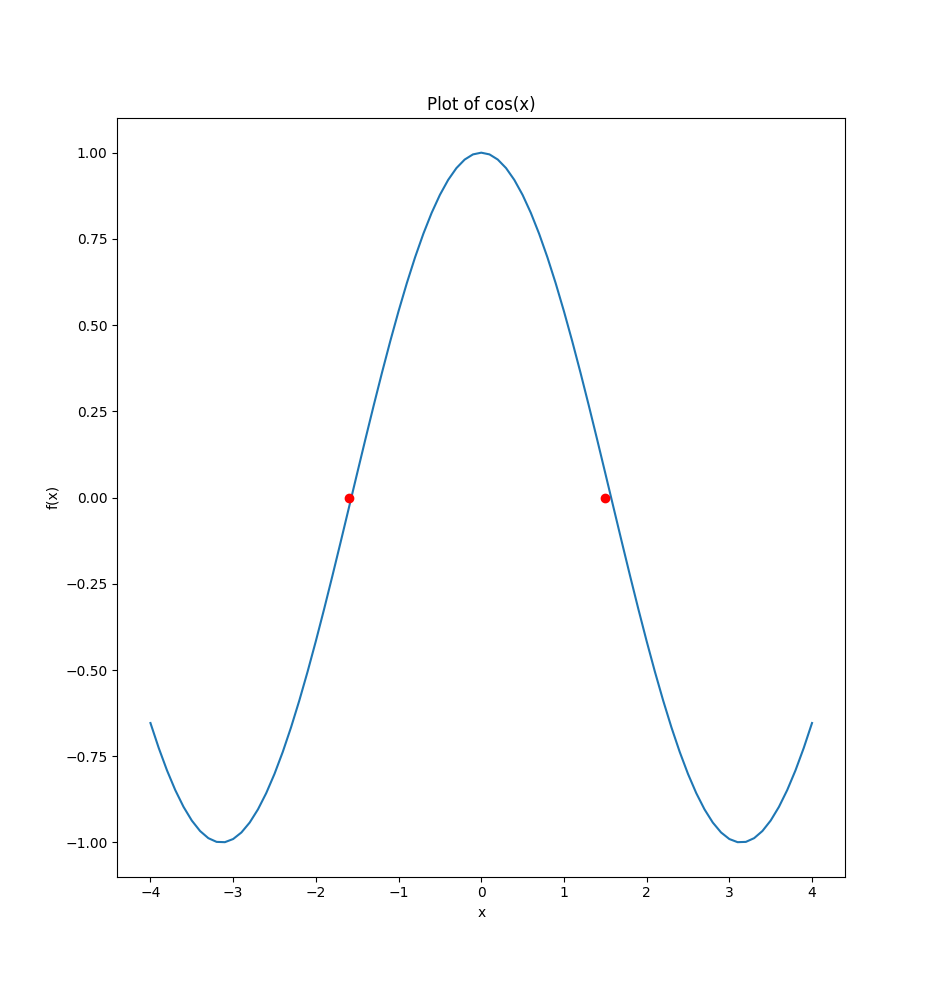
\includegraphics{Figure_1.png}
    \caption{Plot of cos(x)}
    \label{fig:cos}
\end{figure}

\begin{figure}[h]
    \centering
    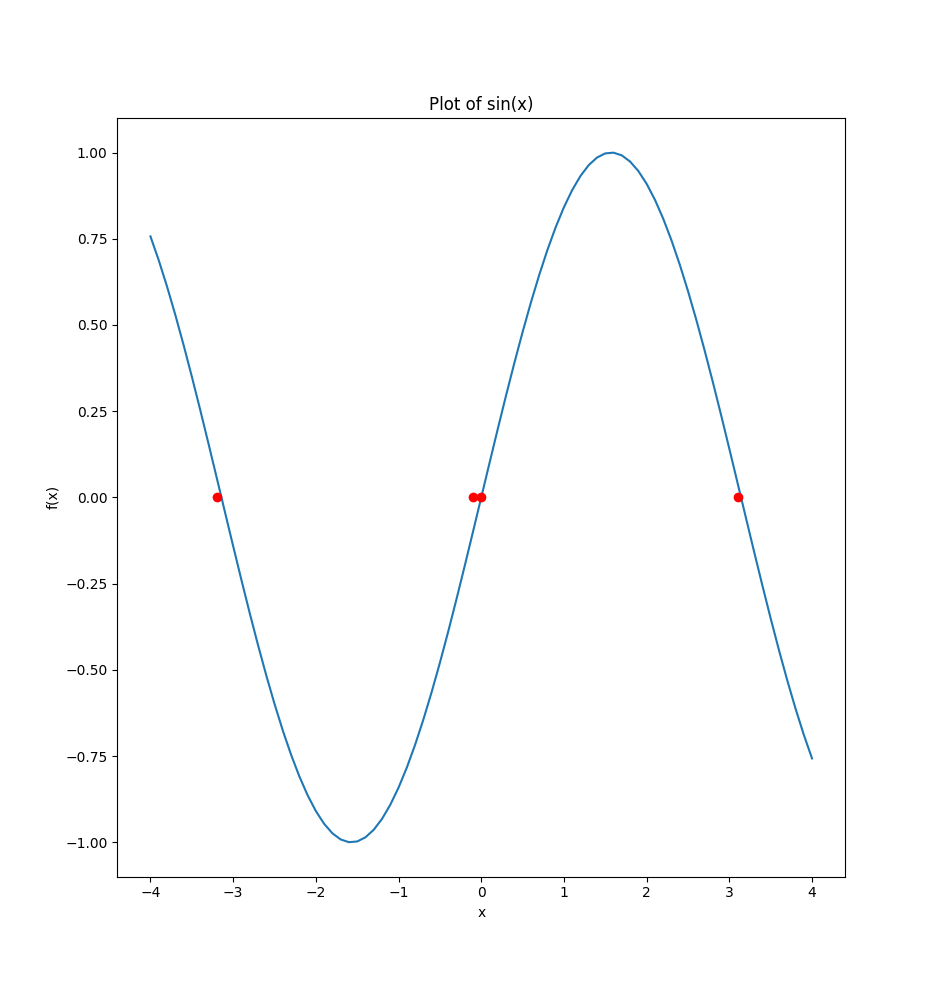
\includegraphics{Figure_2.png}
    \caption{Plot of sin(x)}
    \label{fig:sin}
\end{figure}

\begin{figure}[h]
    \centering
    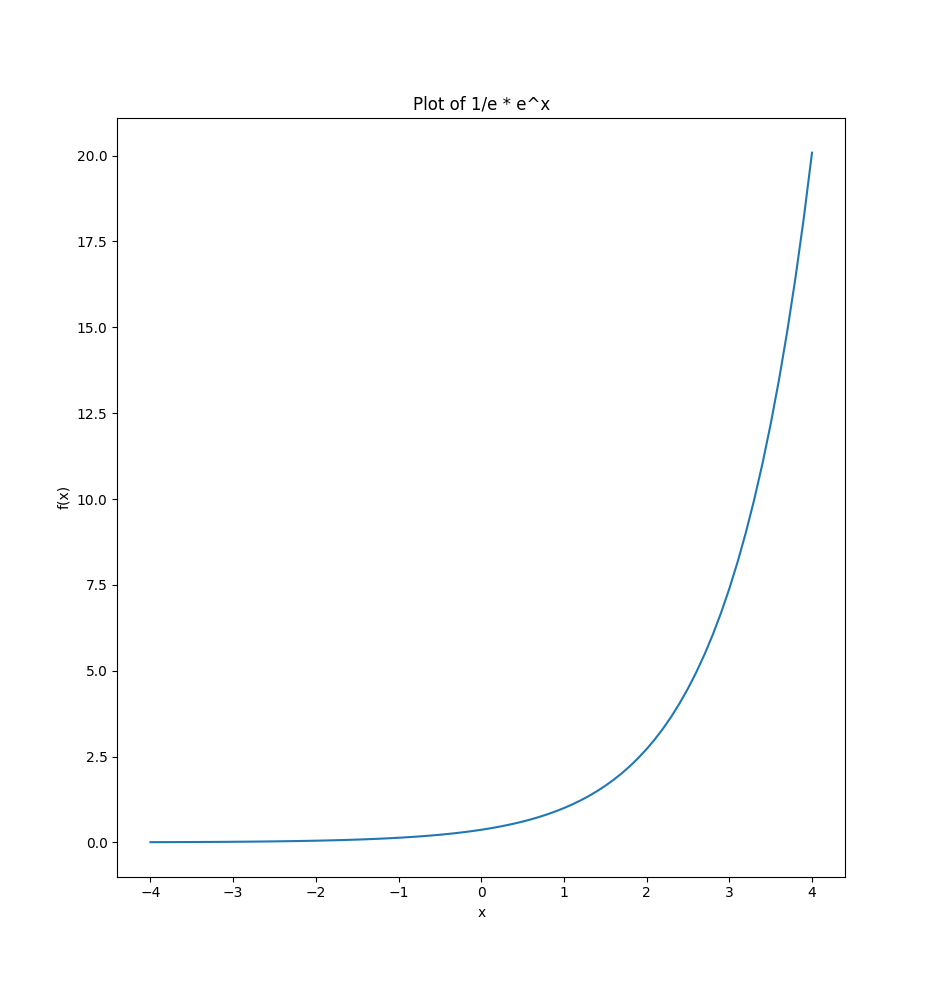
\includegraphics{Figure_3.png}
    \caption{Plot of $\frac{1}{e}e^x$}
    \label{fig:e}
\end{figure}

\begin{figure}[h]
    \centering
    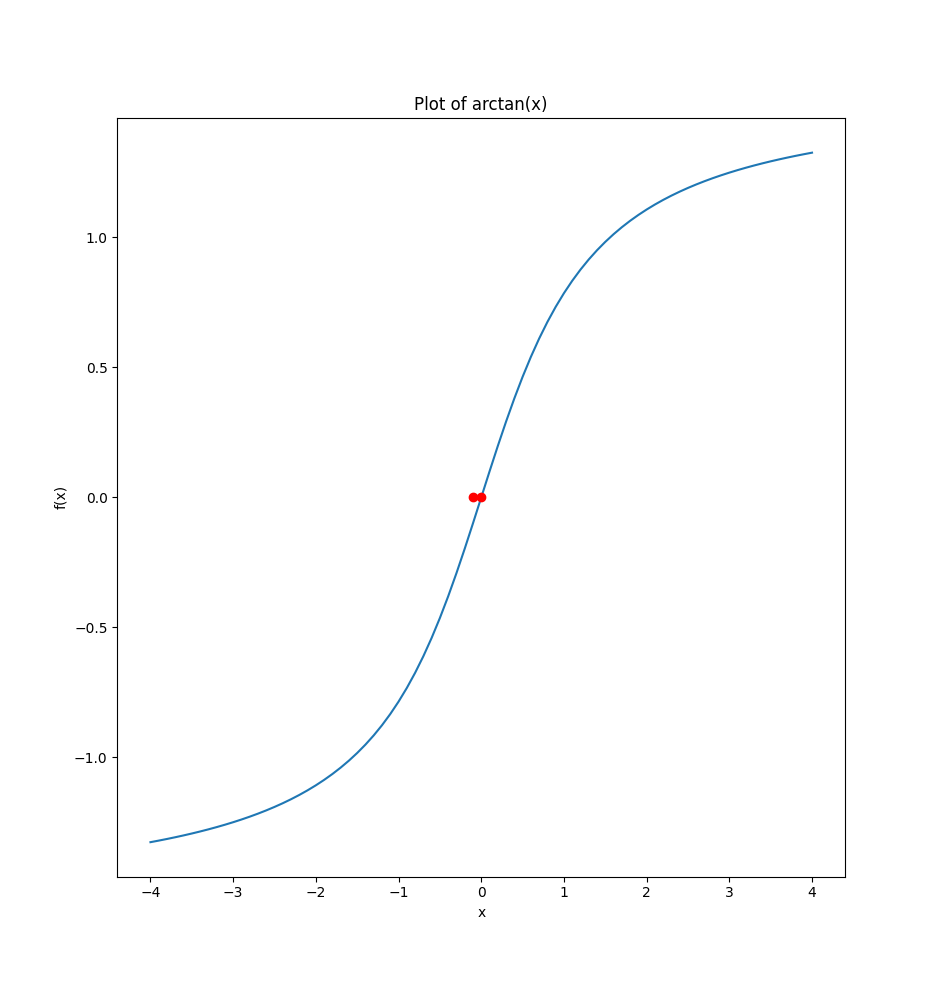
\includegraphics{Figure_4.png}
    \caption{Plot of arctan{x}}
    \label{fig:arctan}
\end{figure}



\begin{figure}[h!]
    \centering
    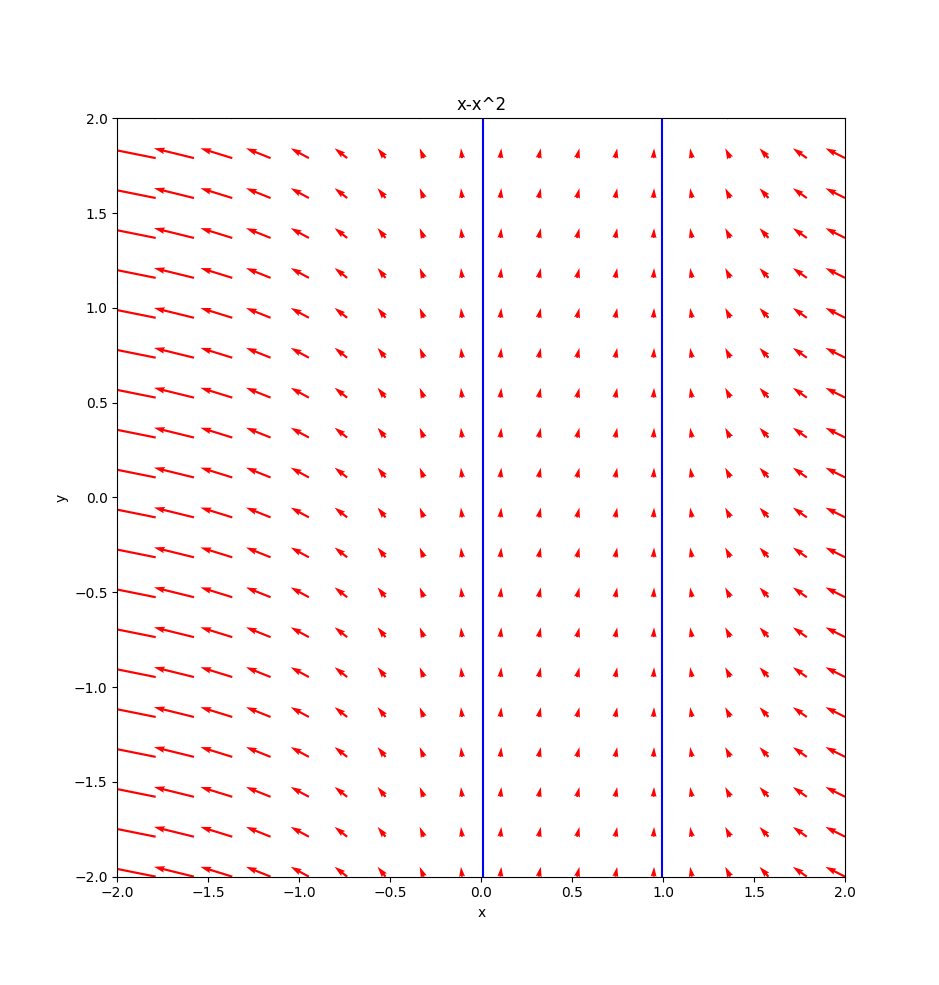
\includegraphics{phase1.png}
    \caption{Phase portrait of $f(x) = x − x^2$}
    \label{fig:phase1}
\end{figure}

\begin{figure}[h!]
    \centering
    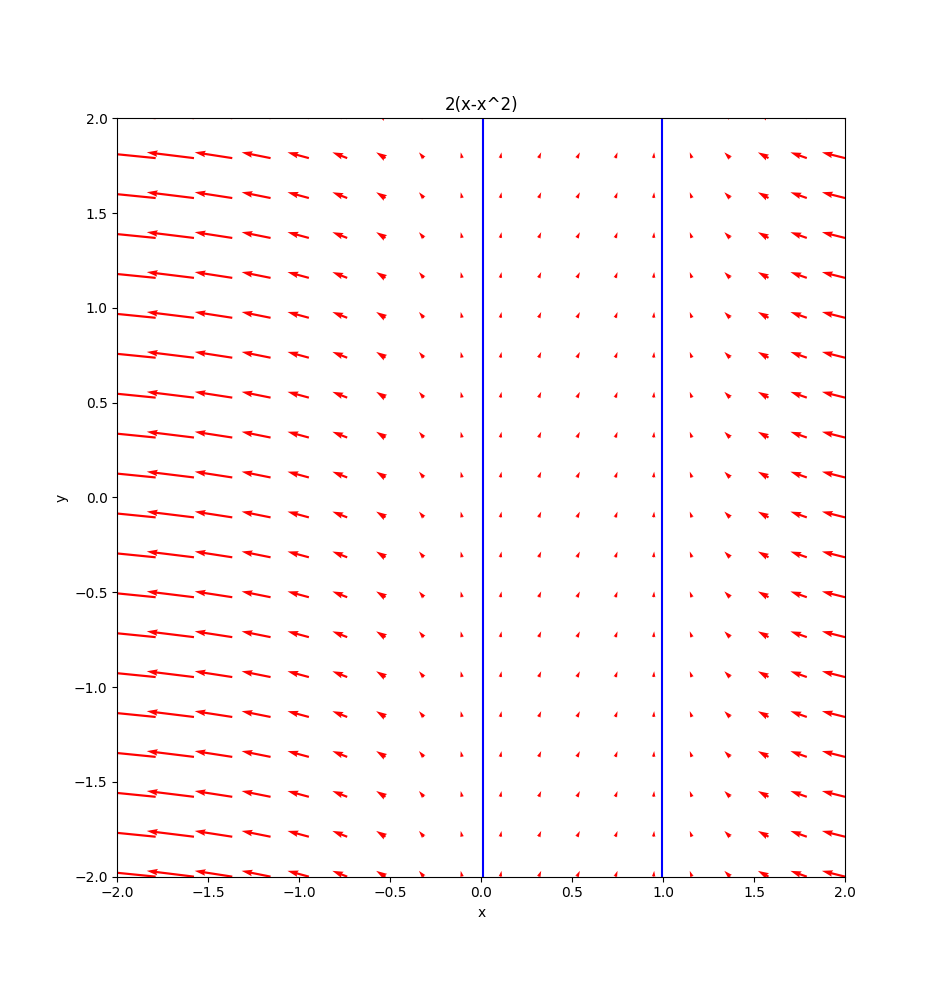
\includegraphics{phase2.png}
    \caption{Phase portrait of $f(x) = 2(x − x^2)$}
    \label{fig:phase2}
\end{figure}

\begin{figure}[h!]
    \centering
    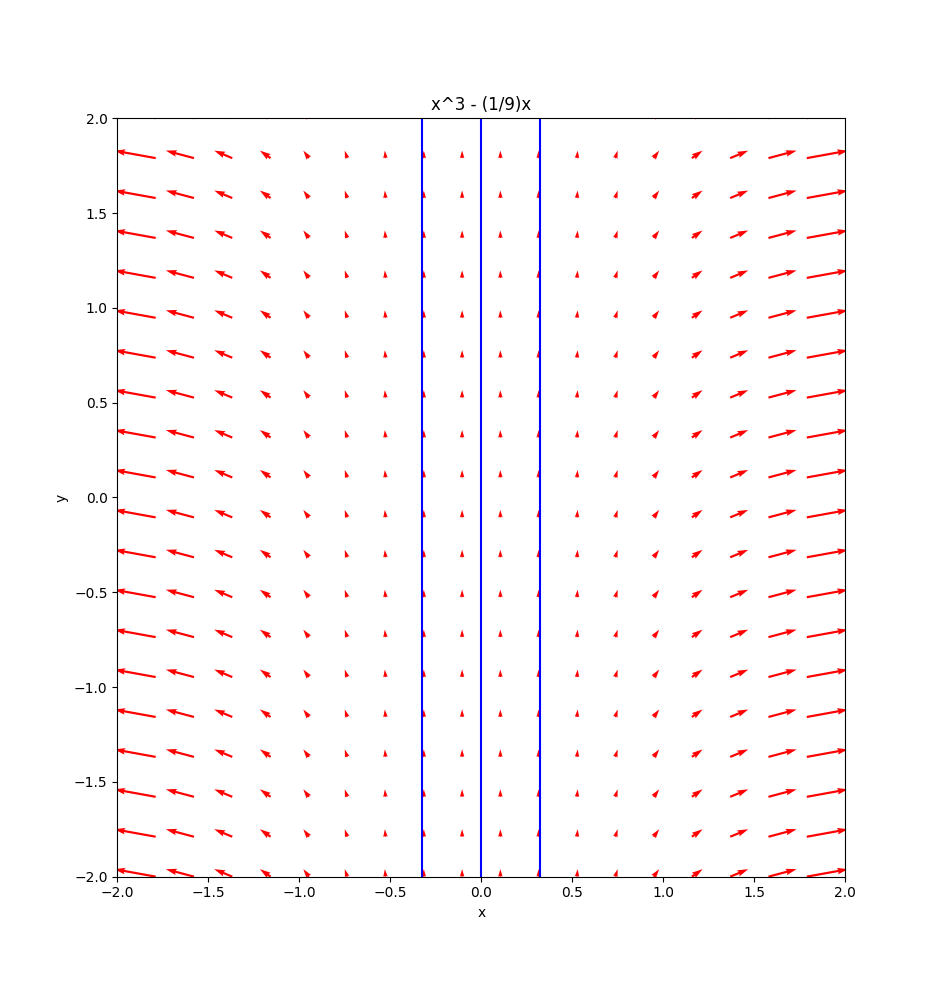
\includegraphics{phase3.png}
    \caption{Phase portrait of $f(x) = x^3 − \frac{1}{9}x$}
    \label{fig:phase3}
\end{figure}

\begin{figure}[h!]
    \centering
    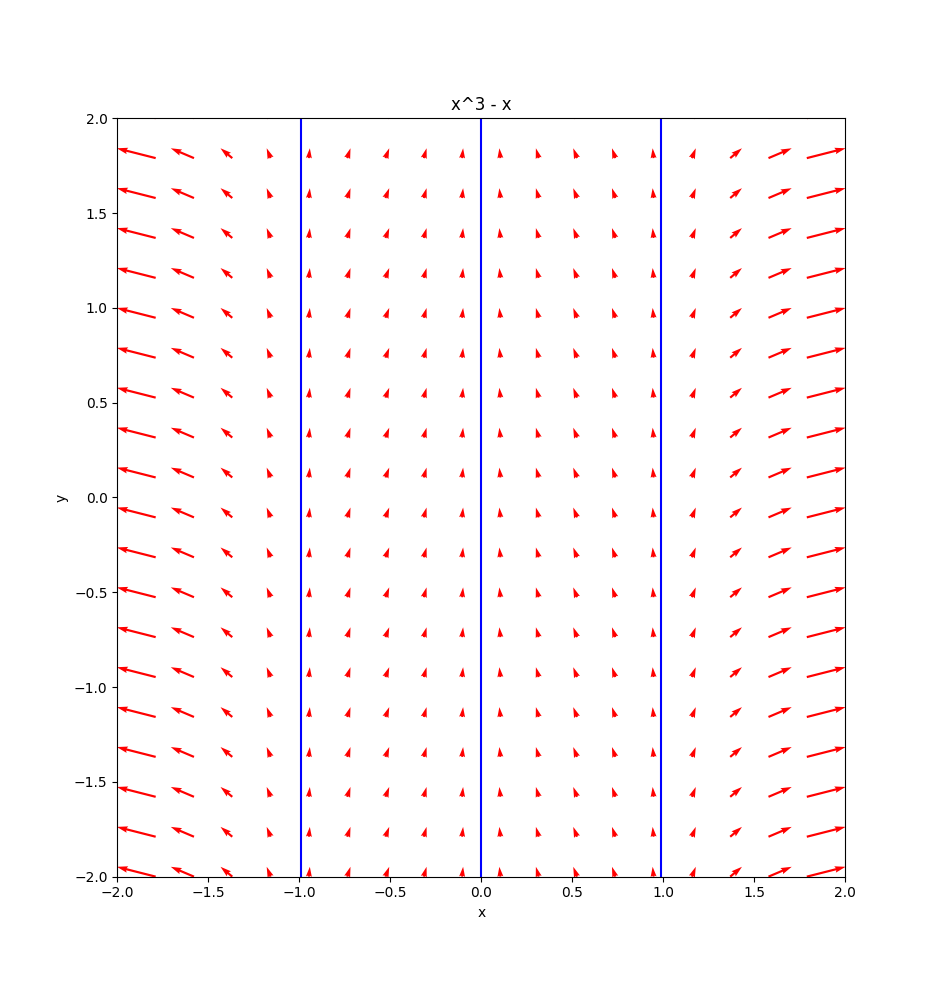
\includegraphics{phase4.png}
    \caption{Phase portrait of $f(x) = x^3 − x$}
    \label{fig:phase4}
\end{figure}

\begin{figure}[h!]
    \centering
    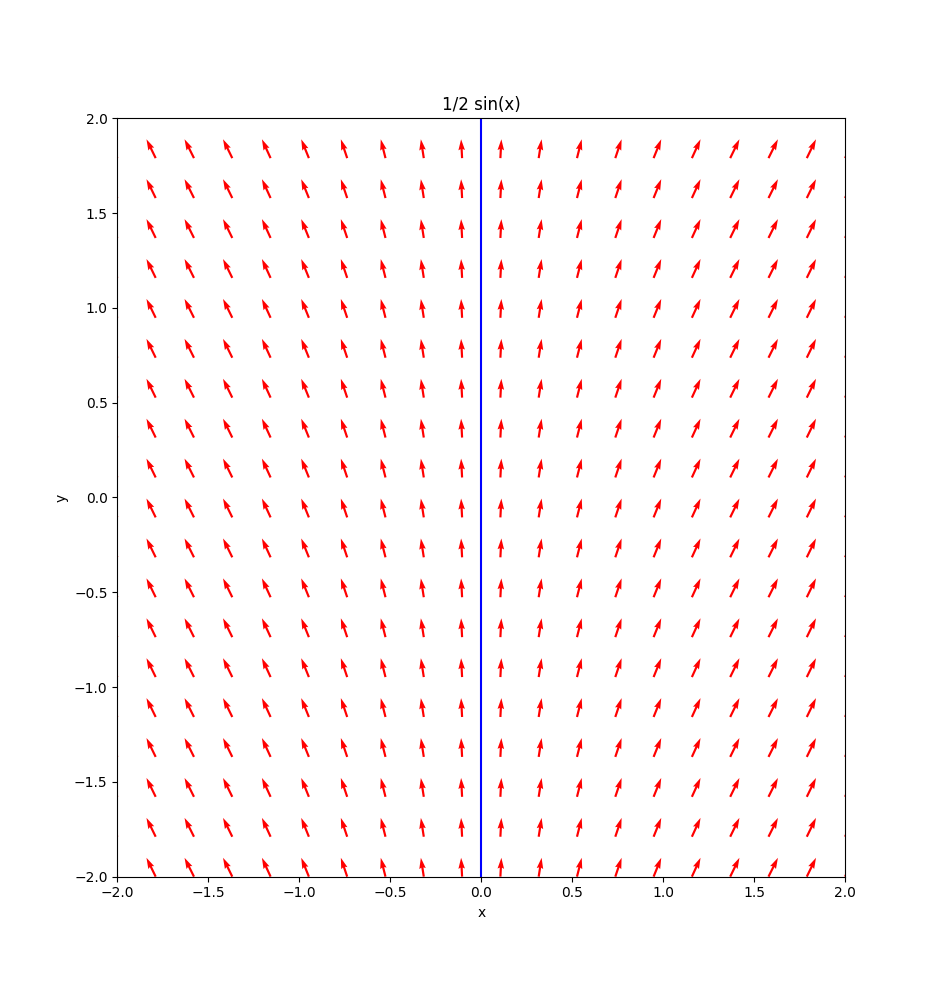
\includegraphics{phase5.png}
    \caption{Phase portrait of $S(x) = \frac{1}{2}sin(x)$}
    \label{fig:phase5}
\end{figure}
    
\begin{figure}[h!]
    \centering
    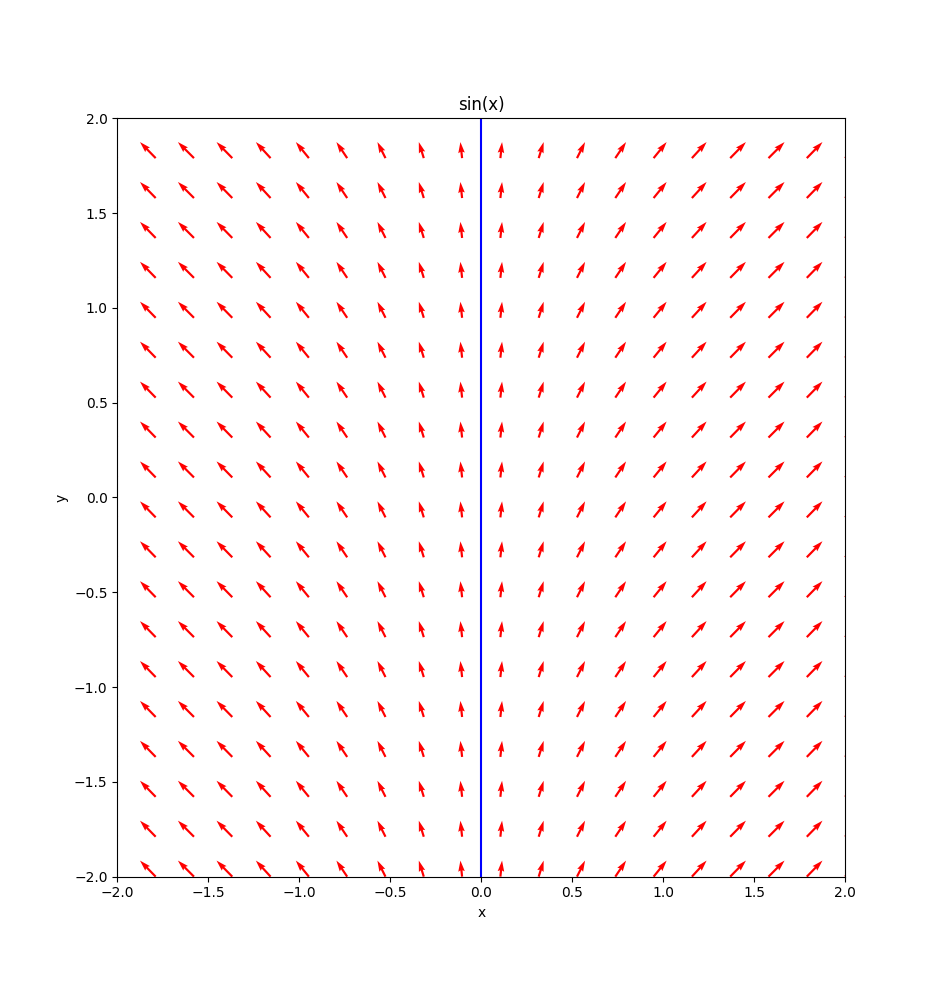
\includegraphics{phase6.png}
    \caption{Phase portrait of $S(x) = sin(x)$}
    \label{fig:phase6}
\end{figure}

\begin{figure}[h!]
    \centering
    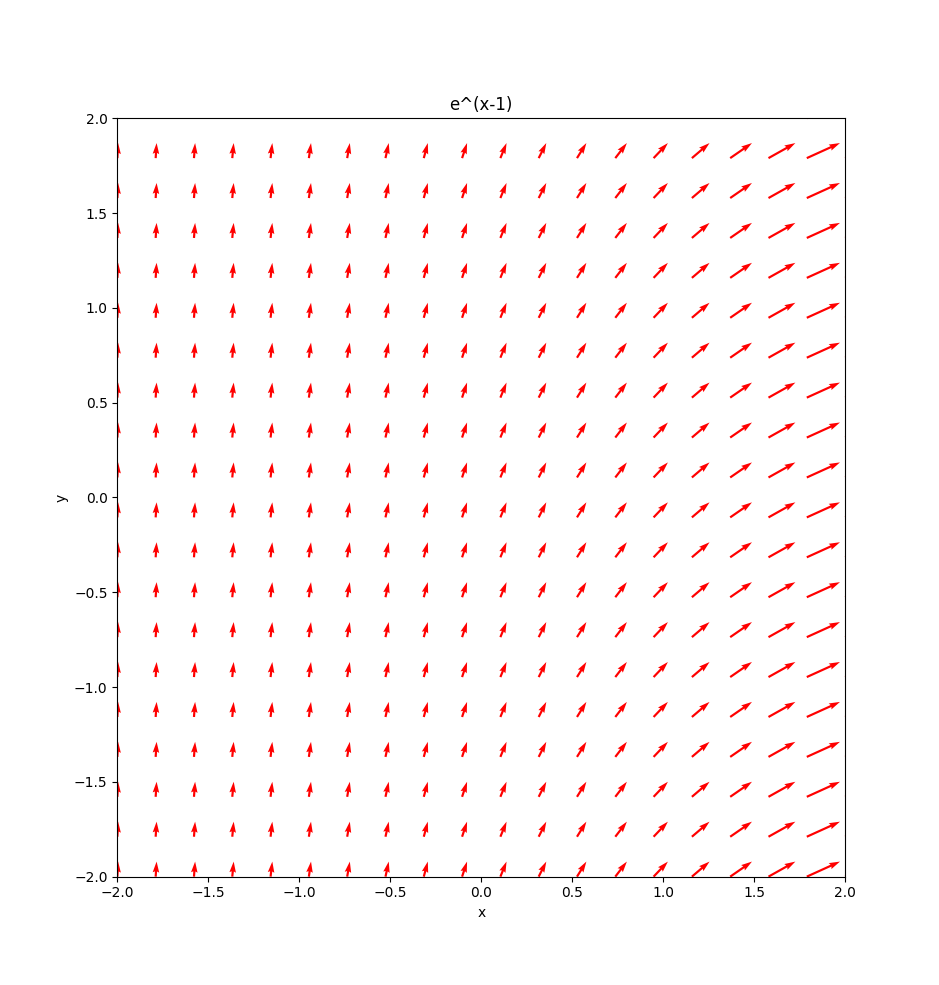
\includegraphics{phase7.png}
    \caption{Phase portrait of $E(x) = e^{x-1}$}
    \label{fig:phase7}
\end{figure}

\begin{figure}[h!]
    \centering
    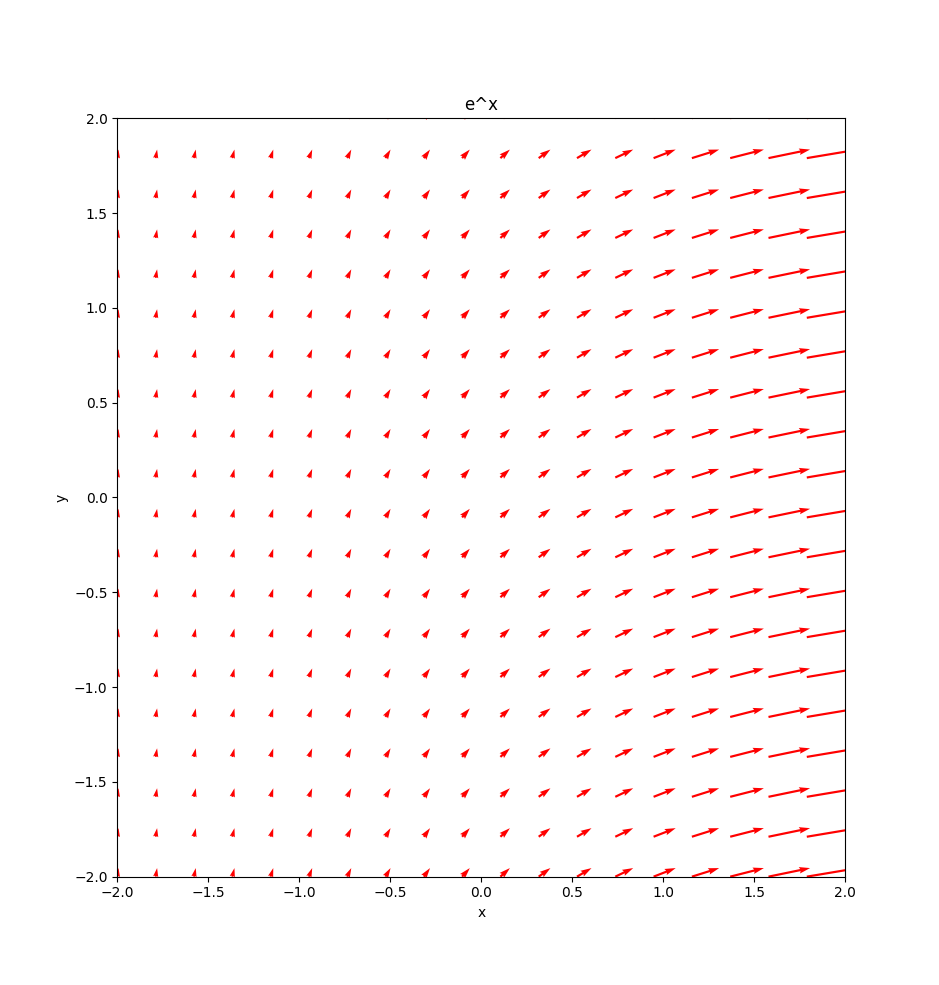
\includegraphics{phase8.png}
    \caption{Phase portrait of $E(x) = e^x$}
    \label{fig:phase8}
\end{figure}

\begin{figure}[h!]
    \centering
    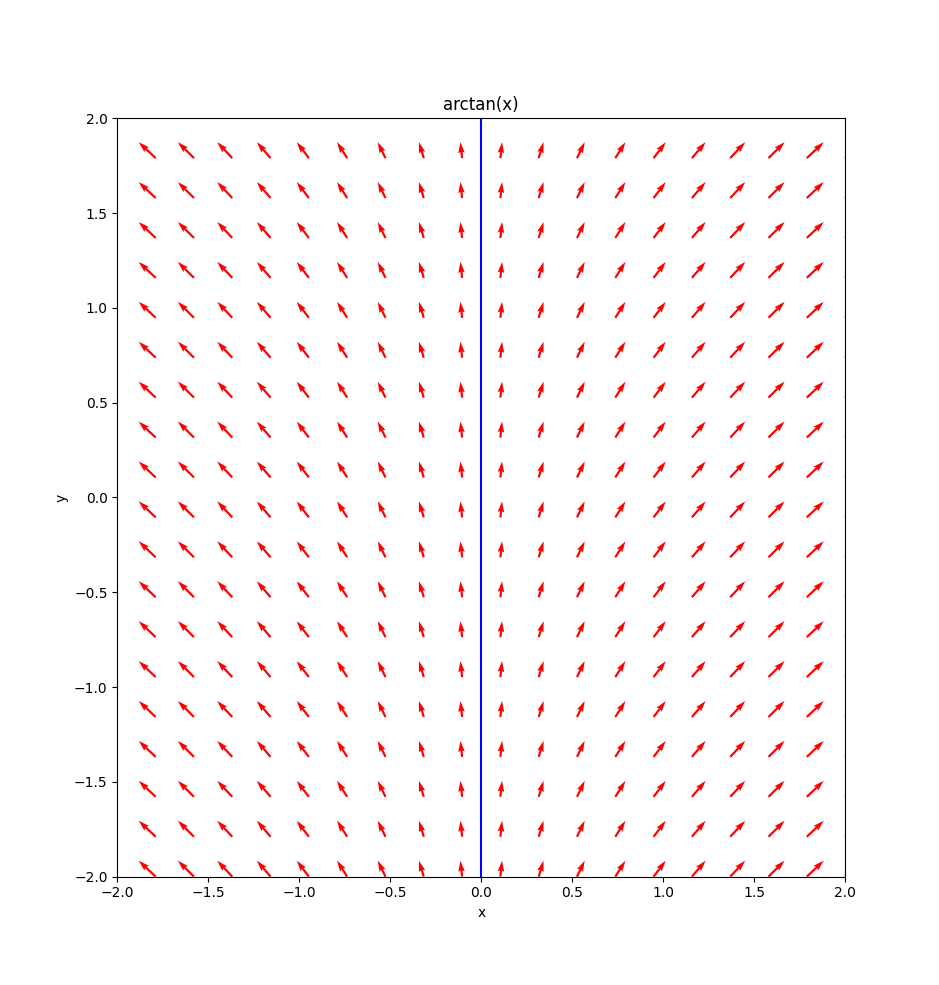
\includegraphics{phase9.png}
    \caption{Phase portrait of $A(x) = arctan(x)$}
    \label{fig:phase9}
\end{figure}

\begin{figure}[h!]
    \centering
    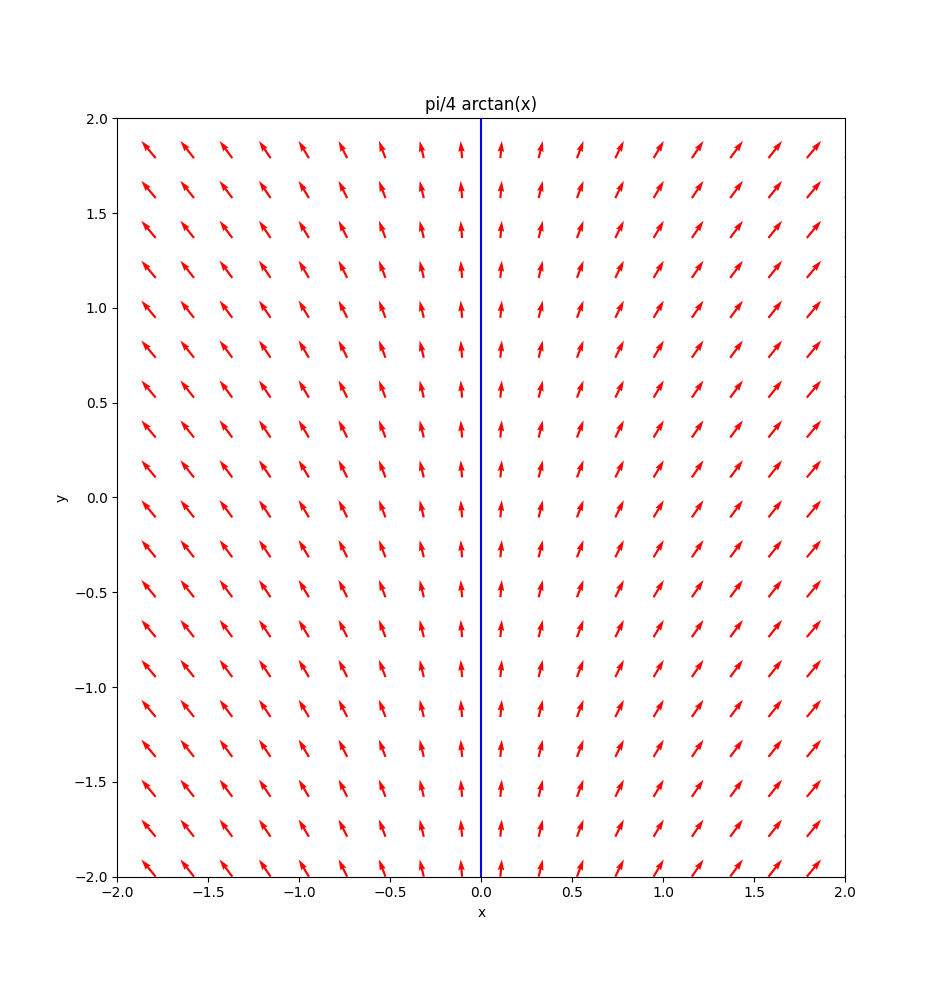
\includegraphics{phase10.png}
    \caption{Phase portrait of $A(x) = \frac{\pi}{4}arctan(x)$}
    \label{fig:phase10}
\end{figure}

\begin{figure}[h!]
    \centering
    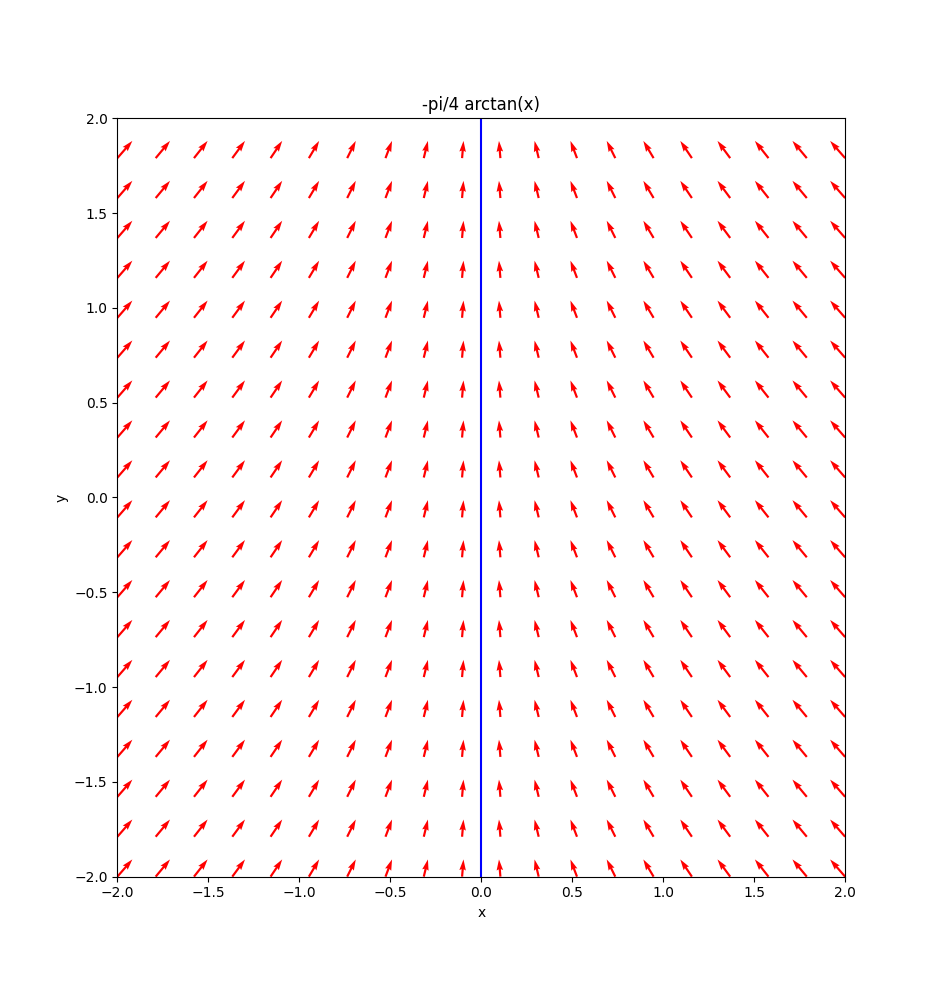
\includegraphics{phase11.png}
    \caption{Phase portrait of $A(x) = -\frac{\pi}{4}arctan(x)$}
    \label{fig:phase11}
\end{figure}

\begin{figure}[h!]
    \centering
    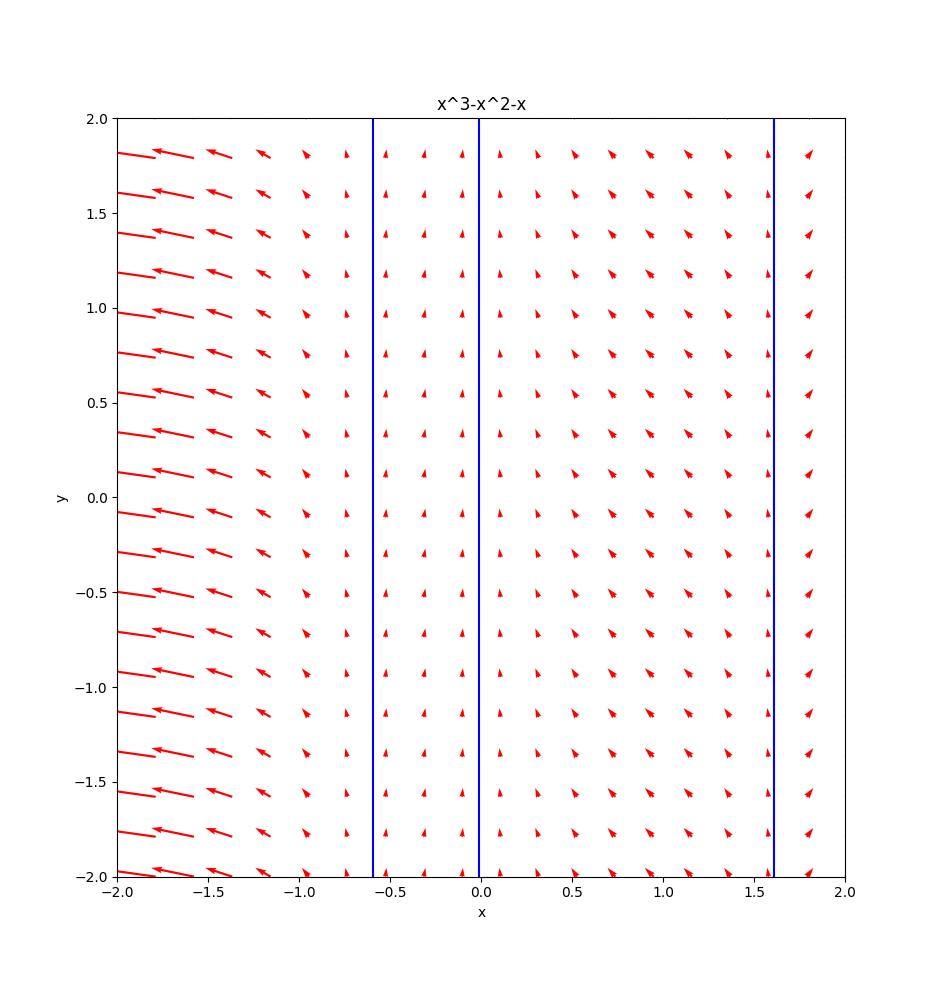
\includegraphics{phase12.png}
    \caption{Phase portrait of $f(x) = x^3 - x^2 -x$}
    \label{fig:phase12}
\end{figure}

\begin{figure}[h!]
    \centering
    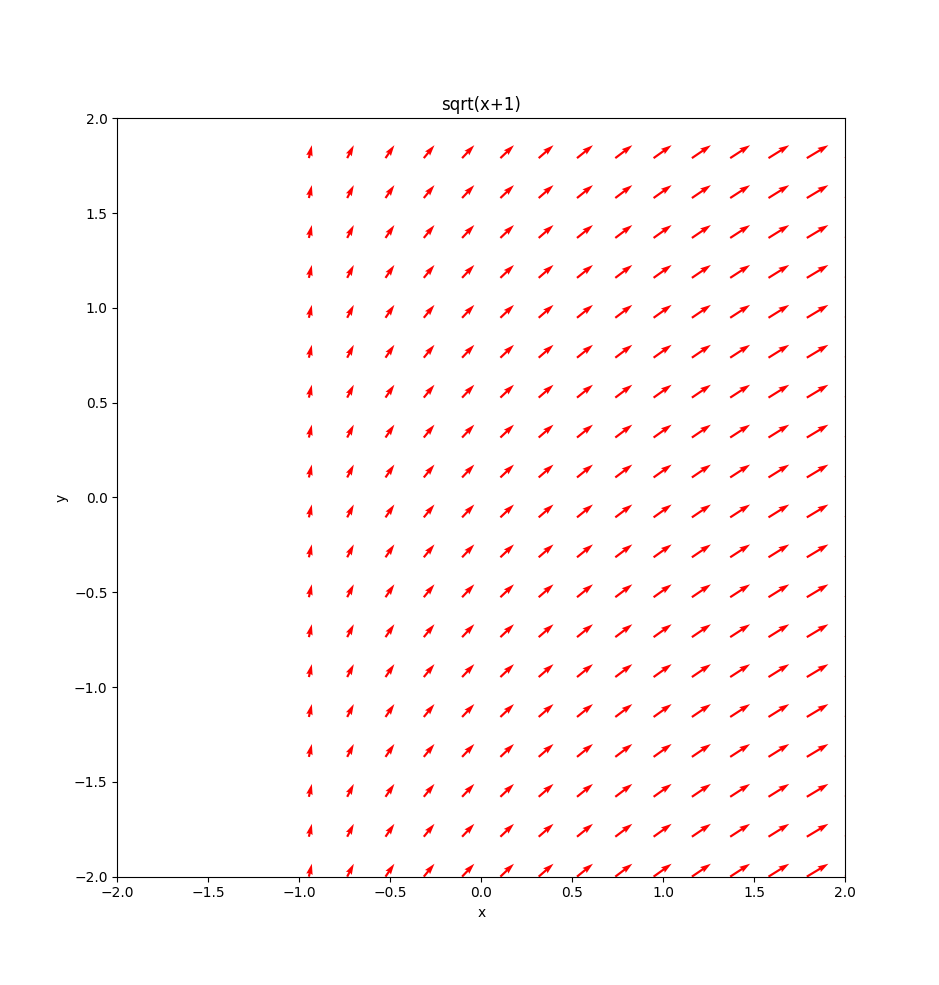
\includegraphics{phase13.png}
    \caption{Phase portrait of $g(x) = \sqrt{x+1}$}
    \label{fig:phase13}
\end{figure}

\begin{figure}[h!]
    \centering
    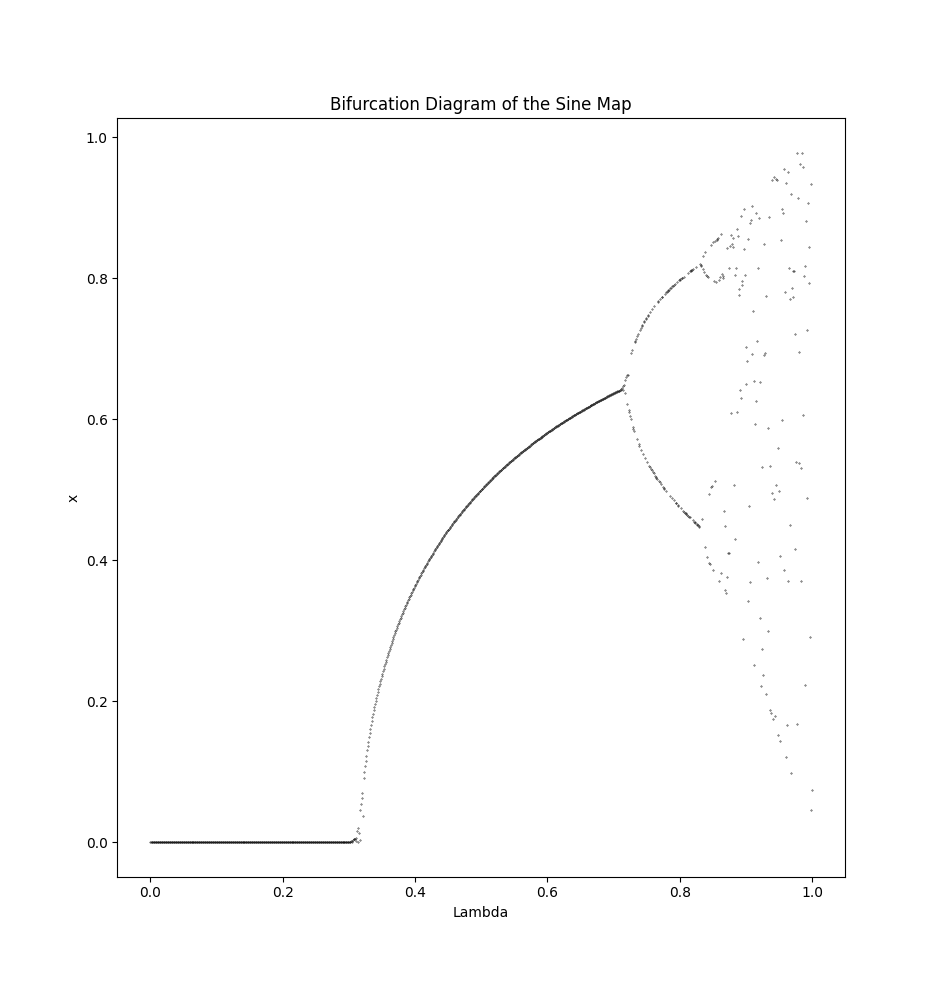
\includegraphics{bifurc.png}
    \caption{Sine map for $\lambda$}
    \label{fig:bifurc}
\end{figure}
\end{document}
